\chapter{Editor's postface}

\emph{The Anatomy of Melancholy} was Burton's life's work. After it was first published he continued editing and improving on it until his death. His last re-edition was published post-humously in 1651. Since melancholy was so dear to Burton it's clear this book was intended not just as work for work's sake but a \mymarginnote{Thucydides, \emph{History of the Peloponnesian War}, Book \rn{I}, 1.22-4.}\textgreek{κτῆμα ἐς ἀεί}\inlinetrans{possession for all time}. The amount of marginalia and inline latin interspersed in the mostly English text make this a difficult book to read, let alone typeset.

It is my sincere hope this edition makes reading the \emph{Anatomy} a bit easier, and that you, the Reader, be touched by the sincere humanity and passion of this melancholic voice from centuries ago. While working on this edition, as Burton saith \mymarginnote{\autopageref{mention:being-busy}.}\textquote{by being busy to avoid melancholy}, I experienced a deep empathy for Burton: melancholy troubled him like so many others and he suffered it with the spirit of inquiry and pursuit of understanding.

Despite his archaic and at times \mymarginnote{like for example listing fishes one should avoid, \autopageref{sec:fishes}.}unintentionally funny approach to the subject the \emph{Anatomy} includes timeless observations and thoughts on the human condition in general, observed through the lens of being melancholy. The myriad quotations and references to the classics and contemporary literature will satisfy the medievalist and classicist readers.

\section*{Presentation of text}

\begin{figure}[H]%
  \centering
  \qquad\begin{minipage}{0.3\textwidth}%
    \frame{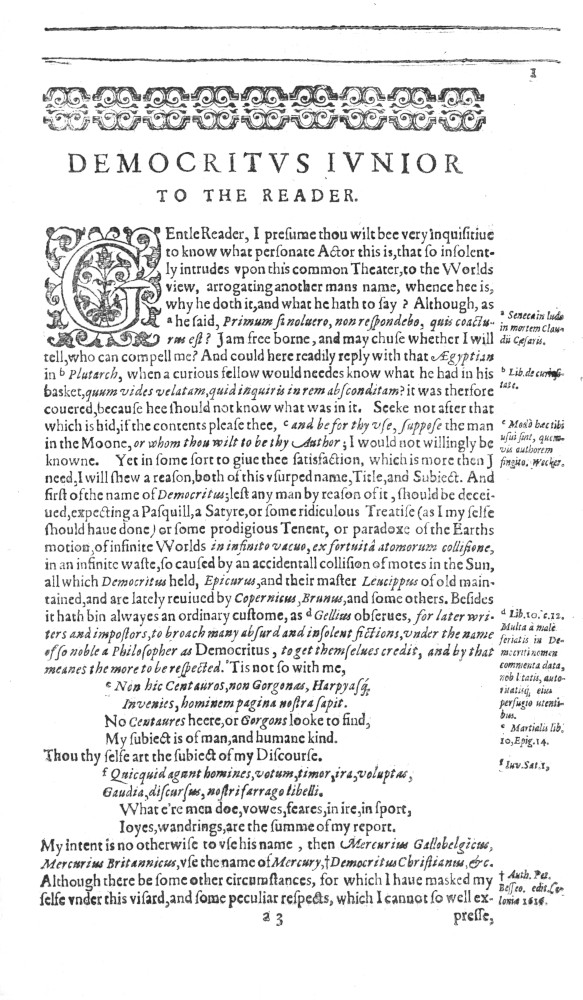
\includegraphics[quiet=true,keepaspectratio]{figures/first-page-first-edition-small.jpg}}
    \caption*{\scriptsize{}\notefont{}First page.}
  \end{minipage}%
  \qquad\begin{minipage}{0.3\textwidth}%
    \frame{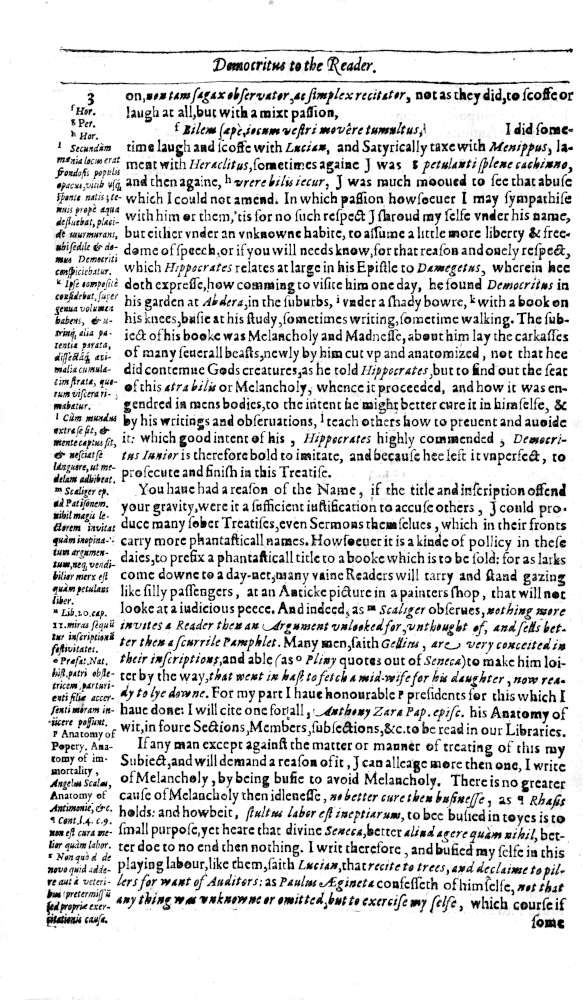
\includegraphics[quiet=true,keepaspectratio]{figures/marginalia-page-first-edition-small.jpg}}
    \caption*{\scriptsize{}\notefont{}Marginalia.}
  \end{minipage}%
  \caption*{Pages from the first edition (1621).}%
  \label{fig:first-edition}%
\end{figure}

In the first edition, every note was placed in the margin. The large textblock and lack of empty space in general make the page very hard to parse. I first encountered the \emph{Anatomy} when I purchased the modern edition published (in 2001) by \mymarginnote{Robert Burton, \emph{The Anatomy of Melancholy}, introduction by William H. Gass (New York Review Books, 2001), \textsc{ISBN}:~978-0-0940322-66-0.}\emph{\textsc{New York Review Books}}, which had all notes pushed back at the end of each partition, making it impractical to read the text along with the notes. Setting the notes in the context where they are meant to be seems like a reasonable requirement: the back-and-forth movement necessary for the reading of notes is a defect or even a defacement of the author's intent.

  \newlength{\minipagewidth}
\setlength{\minipagewidth}{0.3\textwidth}
  \newlength{\pageratio}
\setlength{\pageratio}{\dimexpr((\paperheight)/(\paperwidth))\relax}
  \newlength{\minipageheight}
\setlength{\minipageheight}{\dimexpr(\pageratio*\minipagewidth)\relax}
\begin{figure}[H]%
  \centering
  \qquad\begin{minipage}{0.27\textwidth}%
   \frame{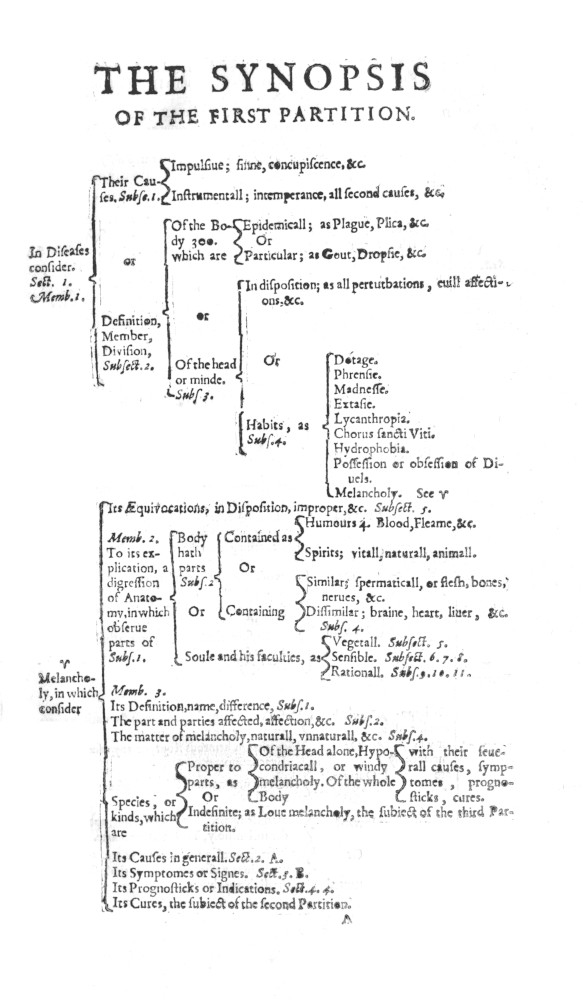
\includegraphics[quiet=true,width=\textwidth,keepaspectratio]{figures/synopsis-schemata-first-edition-small.jpg}}
   \caption*{\scriptsize{}\notefont{}Topical diagram (First edition 1621).}
  \end{minipage}%
  \qquad\begin{minipage}{0.27\textwidth}%
     \begin{minipage}[c][\minipageheight]{\textwidth}%
     \frame{\parbox{\textwidth}{\vspace{\baselineskip}
     {
     \parbox{\textwidth}{\hspace{0.35\textwidth}\resizebox{0.6\textwidth}{!}{\small\textsc{The Synopsis of the First Partition.}}\par
     \vspace{-0.92\baselineskip}
     \hspace{0.15\textwidth}\rule{0.8\textwidth}{.1pt}}\par
     }
     \vspace{0.1\baselineskip}
     \parbox{\textwidth}{\hspace{0.15\textwidth}\resizebox{0.6\textwidth}{!}{\Large{}The Synopsis of the First Partition.}}\par
     \vspace{0.3\baselineskip}
     \parbox{\textwidth}{\hspace{0.15\textwidth}\resizebox{0.8\textwidth}{!}{\SynopsisBoxFirstA}}\par
     \vspace{0.5\baselineskip}
     \parbox{\textwidth}{\hspace{0.15\textwidth}\resizebox{0.8\textwidth}{!}{\SynopsisBoxFirstB}}\par
     \vspace{-0.2\baselineskip}
     \parbox{\textwidth}{\hspace{0.15\textwidth}\resizebox{0.02\textwidth}{!}{\small\pageref{ch:synopsis-of-first-part}\hfill}}\par
     \vspace{0.8\baselineskip}
     \vspace{0.000005\baselineskip}}}
     \caption*{\scriptsize{}\notefont{}\autopageref{ch:synopsis-of-first-part}.}
     \end{minipage}
  \end{minipage}%
 \label{fig:schemata-first-edition}%
\end{figure}

  %\SynopsisBox}
Rendering a book digitally allows the automatic management of references and cross-references. For example, the table of contents, figures, the calculation of page number for cross-references \etc{} are all computed programmatically. Navigating the 1621 edition required consulting the index in the end of the book and the diagrams of topics in the beginning of each partition. For reasons of being thorough and of course aesthetics, they were recreated in \LaTeX{} with the \href{https://www.ctan.org/pkg/schemata}{\myuline{blue}{\texttt{schemata}}} package.

\begin{figure}[H]%
  \centering
    \frame{
\includegraphics[width=\textwidth,quiet=true,keepaspectratio]{figures/chaucer-blackletter-detail.jpg}}
    \caption*{\scriptsize{}\notefont{}Chaucer quotation (First edition 1621). See \autopageref{mention:chaucer-quote-postface}.}
  \label{fig:chaucer-first-edition}%
\end{figure}

Quotations in the 1621 edition were mostly rendered in a cursive typeface (chancery hand), with the exception of \mymarginnote{
  \newlength{\ChaucerPortraitHeight}
  \newsavebox{\ChaucerPortraitBox}
  \savebox{\ChaucerPortraitBox}{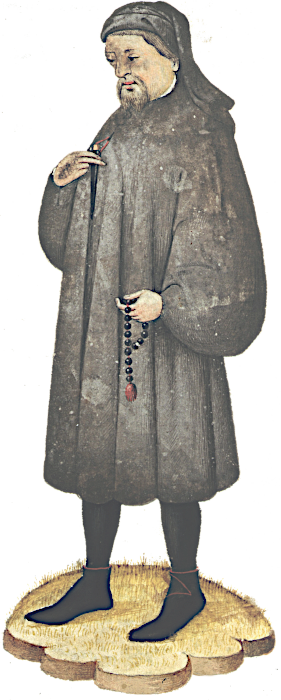
\includegraphics[width=0.4\marginparwidth,quiet=true,keepaspectratio]{figures/Chaucer-small.png}}
  \settoheight{\ChaucerPortraitHeight}{\usebox{\ChaucerPortraitBox}}
  \vspace*{-\ChaucerPortraitHeight-2\baselineskip}
  \par{\noindent\hfil\usebox{\ChaucerPortraitBox}\hfil\par
    \vspace*{\baselineskip}
  Geoffrey Chaucer, English author. Born ca. 1340, died in 1400. Known for \emph{The Canterbury Tales} (1380s), he was influential in establishing vernacular English as a literary language.}}Chaucer whose prose is in \li{textualis formata}, nowadays colloquially known as \emph{Blackletter}. Perhaps the publisher or Burton himself wished to stress the antiquity of Chaucer -a difference of about two centuries- or just follow tradition, as Chaucer's works were first published in this script. For this purpose, this edition uses the \href{https://ctan.org/pkg/ygoth}{\myuline{blue}{\texttt{ygoth}}} typeface by Yannis Haralambous for the same effect.

\clearpage{}
\thispagestyle{titleontop}
\vspace*{\fill} 
\begin{quote} 
\centering 
{\huge\textquote{Be not solitary,\\ be not idle.}}
\end{quote}
\vspace*{\fill}

